\chapter{Knowledge acquired}

During the time of this project, I have learnt many things, from non-technical to technical, such as teamwork, communication, code re-used, code convention. 

\section{Design Pattern}

Code re-used is an important factor in software development industry. You can work faster or not depends on how good your code re-using skill is. And design pattern is a part of code re-used. In the project, there are some views that were used in many screens. At first I repeat the same implementing process everytime, and the code for each screen grow quite big. That's when I started to use design pattern, and suprisingly, it work well.


\begin{figure}[H]
\centering
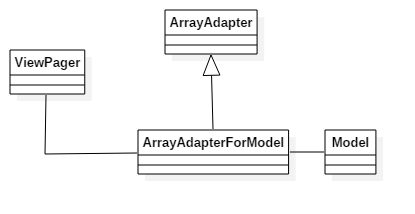
\includegraphics[scale=0.7]{ClassDiagram1}
\caption{Class diagram for normal use of ViewPager}
\end{figure}

\textit{ViewPager} is a view provided by Android, it's used to perform slide action when there'are many images, or sections. Above is a class diagram when normally implementing ViewPager. An instance of \textit{Model} is a data object that we want to present it within \textit{ViewPager}. So if we have many class \textit{Models}, we have to rewrite \textit{ArrayAdapter} corresponding to each \textit{Model}. So my first approach is below :

\begin{figure}[H]
\centering
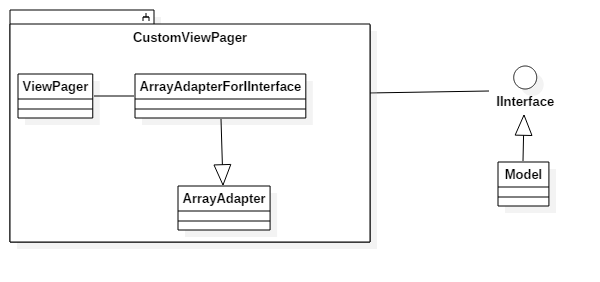
\includegraphics[scale=0.7]{ClassDiagram2}
\caption{First approach}
\end{figure}

With this approach, my code reduce significantly. I just have to write some more functions defined in \textit{IInterface} for \textit{Model}. But then there's another problem. I have to rewrite some classes \textit{Model} that I had created long before, and everyone were working on it, so modifying existed file need to be prevented. Then I came up with second approach, based on the first one :

\begin{figure}[H]
\centering
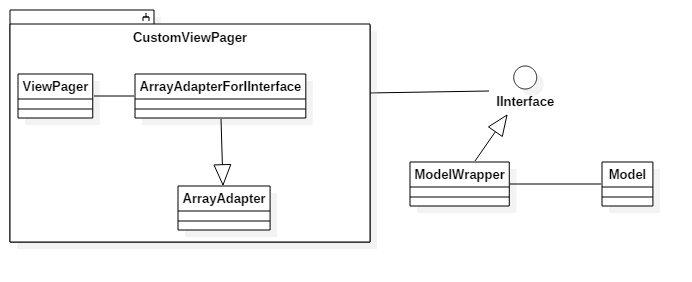
\includegraphics[scale=0.7]{ClassDiagram3}
\caption{Second approach}
\end{figure}

This time, instead of extending class \textit{Model}, I used a medium \textit{ModelWrapper} which envelop \textit{Model} and implement interface \textit{IInterface}. Then each time I want to apply \textit{CustomViewPager} for a new \textit{ModelA}, I just need to create a class \textit{ModelAWrapper} (normally this wrapper had around 20 lines of code).

And after reviewing this scheme, I just realized that I had just apllied \textit{Adapter Pattern} in \textit{Design Pattern}.

\section{Custom View}

Apart from \textit{Design Pattern}, making custom view and re-used it is a great way of re-using code too. In this project, I had made a textview in which the text is align with the diagonal of the textview's bound, a circle view which has shadow, and a layout with shadow. 

Custom component could make your work easier, depend on how convenient it became. In Android, a \textit{Spinner} is a dropdown combo box, which let user choose an item from its dropdown list. The normal way of using such component, is to enter a list of \textit{String}, and when user choose one item, this \textit{Spinner} will return the position of the selected item, and then we can retrieve the corresponding object. 

\begin{figure}[H]
\centering
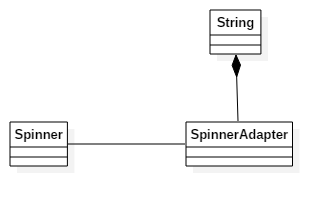
\includegraphics[scale=0.7]{Spinner1}
\caption{Tradition Spinner}
\end{figure}

Let analize the example below :

I have an array of \textit{Good}, like Candy, Wine, Clothes, etc. If I want to make a \textit{Spinner} using the above method to display good's name, and available quantity, it would be a little more complicated, since each item has 2 values: a name, and a quantity number, but it's still doable. Then if we want to add more functions, such as reduce the quantity, it would mean that we have to clear the data of the \textit{Spinner}, and re-insert the new data each time we updated the data. 

So I came up with another solution. Instead of using the tradition \textit{String} as input for \textit{Spinner}, I decide to use \textit{Good}. And every time an instance of \textit{Good} is updated, its automatically update the \textit{Spinner} as well. And moreover, when I selected an item in the dropdownlist, unlike before, I obtain a \textit{Good}'s instance, instead of a \textit{String}. And that make my work faster and easier. 

\begin{figure}[H]
\centering
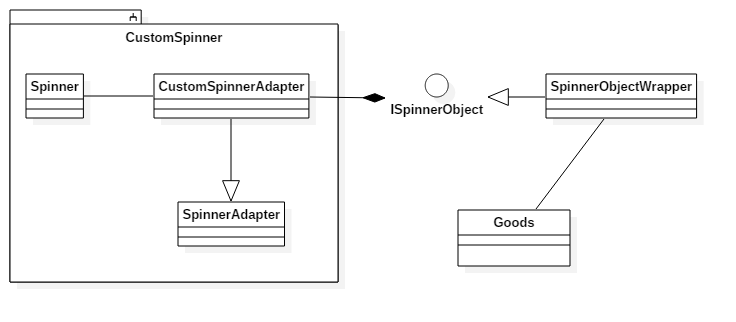
\includegraphics[scale=0.7]{Spinner2}
\caption{My Spinner}
\end{figure}